\documentclass{article}
\usepackage[utf8]{inputenc}
\usepackage[top=1in]{geometry}
\usepackage{tikz}
\usetikzlibrary{circuits.logic.US,positioning,calc} 
\usepackage{graphicx}
\usepackage{booktabs}
\usepackage{amsmath}
\usepackage[colorlinks]{hyperref}
\title{Homework 5}
\author{Max marks: 100}
\date{Due on Oct 31, 2022 (Monday), 12:00 noon, before class. Please submit in paper,
because it is easier to grade. Also submit a backup copy to brightspace.}
\newtheorem{prob}{Problem}

\newcommand{\bx}{\bar{x}}
\newcommand{\by}{\bar{y}}
\newcommand{\bz}{\bar{z}}
\newcommand{\bA}{\bar{A}}
\newcommand{\bB}{\bar{B}}
\newcommand{\bC}{\bar{C}}
\begin{document}

\maketitle

% Appendix B problems 1, 2, 3, 8, 10, 13.
\section{Problems}

\begin{prob}
  A minority gate produces a TRUE output if and only if fewer than
  half of its inputs are TRUE. Otherwise it produces a FALSE output. Sketch a
  transistor-level circuit for a three-input CMOS minority gate. Use a minimum
  number of transistors. (10 marks)
\end{prob}
\begin{prob}
  Write a truth table for the function performed by the gate in
  the figure below. The truth table should have three inputs, A, B, and C. (10
  marks) \\
  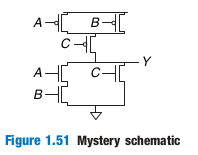
\includegraphics[width=0.3\linewidth]{./fig/fig.1.51-mystery-schematic.png} 
\end{prob}

\begin{prob}
  Consider the circuit shown in Figure PB.1.
  \begin{enumerate}
    \item Write the circuit as a boolean expression for $f$ (5 marks)
    \item Implement the circuit as a CMOS complex gate, how many transistors are
      needed? (15 marks)
    \end{enumerate}
    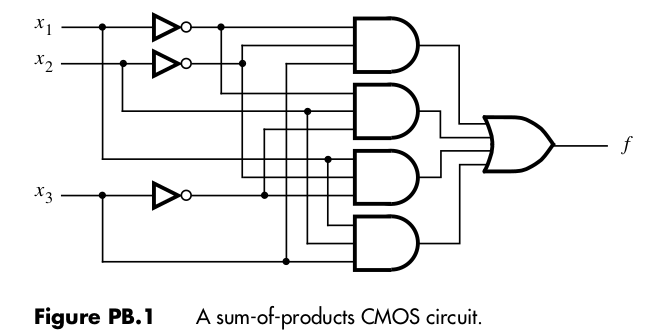
\includegraphics[width=0.6\linewidth]{./fig/figPB.1-SOP-CMOS.png}
\end{prob}
\begin{prob}
  \begin{enumerate}
  \item Show that the circuit in Figure PB.2 is functionally equivalent to the
    circuit in Fig- ure PB.1. (15 marks)
  \item How many transistors are needed to build this CMOS circuit? Assume that
    the multiplexers are built using transmission gates (5 marks).
  \end{enumerate}
  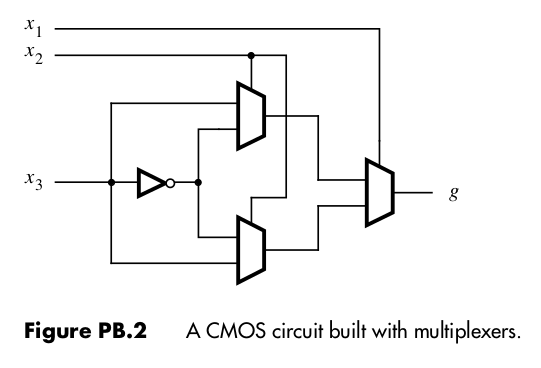
\includegraphics[width=0.6\linewidth]{./fig/figPB.2-CMOS-multiplexer.png}
\end{prob}

\begin{prob}
  Determine the propagation delay and contamination delay of the
  circuit in Figure 2.84. Use the gate delays given in Table 2.8. (10 marks)\\
  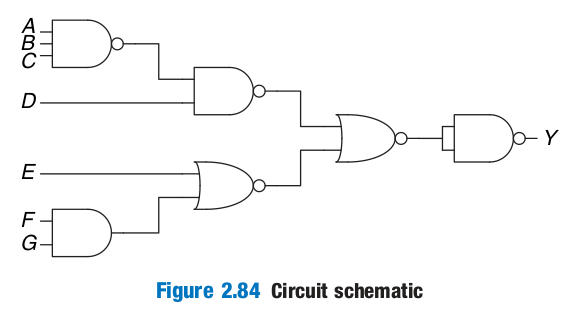
\includegraphics[width=0.4\linewidth]{./fig/fig2.83-circuit.png} 
  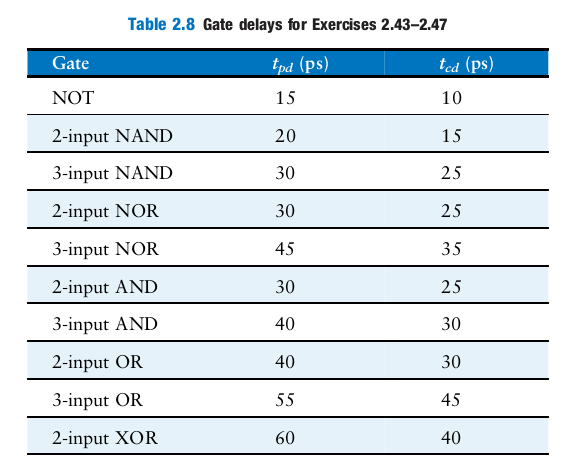
\includegraphics[width=0.4\linewidth]{./fig/tab2.8-gate-delays.png}
\end{prob}

\begin{prob}
  Find a minimal Boolean equation for the function in Figure 2.85.
  Remember to take advantage of the don’t care entries (marked X) (10 marks).
  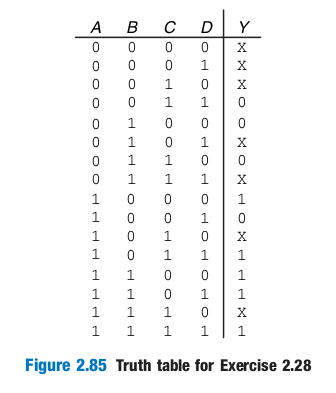
\includegraphics[width=0.3\linewidth]{./fig/fig2.85-truth-table.png}
  \begin{enumerate}
  \item Sketch a circuit for the function (10 marks).
  \item Does your circuit from have any potential glitches
    when one of the inputs changes? If not, explain why not. If so, show how to
    modify the circuit to eliminate the glitches (10 marks).
  \end{enumerate}
\end{prob}
\end{document}